\documentclass[twocolumn, 10pt]{article}
\usepackage[utf8]{inputenc}
\usepackage{ctex} % Support for Chinese characters
\usepackage{geometry}
\geometry{a4paper, margin=1.5cm}
\usepackage{amsmath, amssymb}
\usepackage{booktabs}
\usepackage{graphicx}
\usepackage{cite}
\usepackage{caption}
\usepackage{titlesec}
\usepackage{tikz}
\usetikzlibrary{decorations.markings}

\begin{titlepage}
	\begin{center}
		\vspace*{2cm}
		{\Huge \bfseries 普通物理实验报告 \par}
		\vspace{3cm}
		
		{\huge \bfseries 落球法测量液体粘滞系数的实验研究与误差分析 \par}
		\vspace{4cm}
		
		\doublespacing
		{\Large
			\begin{tabular}{rl}
				\textbf{姓\qquad 名：} & 党佳一 \\
				\textbf{学\qquad 号：} & 202511101093 \\
				\textbf{学\qquad 院：} & 物理与天文学院 \\ % 可根据实际情况修改
				\textbf{实验时间：} & 2026年4月26日 \\
			\end{tabular}
		}
		\singlespacing
		
		\vfill
		{\Large \textbf{北京师范大学物理与天文学院} \par}
		\vspace{2cm}
	\end{center}
\end{titlepage}

% Title styling
\title{\vspace{-1cm}\textbf{落球法测量液体粘滞系数的实验研究与误差分析}}
\author{北京师范大学物理与天文学院}
\date{\today}

\titleformat{\section}{\large\bfseries}{\thesection}{1em}{}
\titleformat{\subsection}{\normalsize\bfseries}{\thesubsection}{0.5em}{}

\begin{document}
	
	\maketitle
	
	\begin{abstract}
		本实验采用落球法测量特定液体的粘滞系数。实验中利用螺旋测微计精确测量小球直径，通过光电门计时装置获取小球在液体中的收尾速度。在数据处理过程中，引入了Oseen修正项以补偿雷诺数（$Re > 0.1$）引起的惯性力偏差，并结合Ladenburg公式对圆筒壁面效应和底面效应进行了边界修正。实验结果表明，在$23.5^\circ\text{C}$环境下，测得液体粘滞系数为 $0.726 \text{ Pa}\cdot\text{s}$，与理论模型具有良好的一致性。
		\\[2mm]
		\textbf{关键词：} 落球法；粘滞系数；Oseen修正；Ladenburg修正；收尾速度
	\end{abstract}
	
	\section{引言}
	液体粘滞系数（内摩擦系数）是表征液体流动特性的重要物理量。在低雷诺数流动中，小球受到的粘滞阻力遵循斯托克斯定律（Stokes' Law）。然而，在实际物理实验中，容器的有限尺寸以及流体惯性对斯托克斯定律的偏离不容忽视。本实验旨在通过修正模型，探索提高液体粘滞系数测量精度的方法。
	
	\section{实验原理}
	
		\begin{center}
		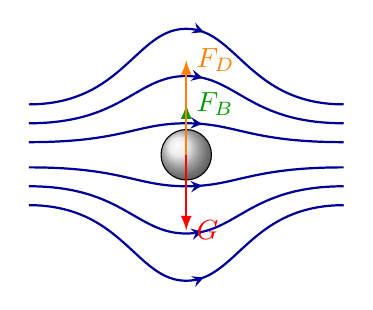
\begin{tikzpicture}[scale=0.8]
			% 绘制小球
			\shade[ball color=gray!20] (0,0) circle (0.4cm);
			\draw (0,0) circle (0.4cm);
			
			% 绘制对称的流线
			\foreach \y in {-0.8,-0.5,-0.2,0.2,0.5,0.8} {
				\draw[blue!60!black, thick, postaction={decorate, decoration={
						markings, mark=at position 0.55 with {\arrow{stealth}}}}] 
				(-2.5,\y) .. controls (-1, \y) and (-0.8, \y*2.5) .. (0, \y*2.5)
				.. controls (0.8, \y*2.5) and (1, \y) .. (2.5, \y);
			}
			
			% 标注力
			\draw[-latex, red, thick] (0,0) -- (0,-1.2) node[right] {$G$};
			\draw[-latex, green!60!black, thick] (0,0) -- (0,0.8) node[right] {$F_B$};
			\draw[-latex, orange, thick] (0,0) -- (0,1.5) node[right] {$F_D$};
		\end{tikzpicture}
		\captionof{figure}{受力分析与流线分布示意图}
	\end{center}
	\subsection{斯托克斯公式及其修正}
	当球形物体在无限深广的液体中匀速下落时，其受力平衡方程为：
	\begin{equation}
		\frac{1}{6}\pi d^3 \rho_0 g = \frac{1}{6}\pi d^3 \rho g + F_D
	\end{equation}
	其中 $F_D$ 为粘滞阻力。对于非极低雷诺数的情况，考虑惯性修正后的 $F_D$ 可表示为：
	\begin{equation}
		F_D = 3\pi \eta d v_0 (1 + \frac{3}{16}Re)
	\end{equation}
	由此导出未经边界修正的粘滞系数表达式 $\eta^{(0)}$：
	\begin{equation}
		\eta^{(0)} = \frac{(\rho_0 - \rho)d^2 g - \frac{27}{8}\rho d v_0^2}{18 v_0}
	\end{equation}

	
	\subsection{边界效应修正}
	受圆筒内径 $D$ 和液柱高度 $H$ 的限制，需引入边界修正系数 $k$：
	\begin{equation}
		k = (1 + 2.4 \frac{d}{D})(1 + 1.6 \frac{d}{H})
	\end{equation}
	最终实验测量值为 $\eta = \eta^{(0)} / k$。

	\begin{figure}[htbp]
	\centering
	\includegraphics[width=0.8\linewidth]{C:/Users/党佳一/Pictures/Screenshots/屏幕截图 2026-04-26 124753.png}
	\caption{\centering 测试架结构
		1.落球导管 2.发射端I 3.发射端II 4.量筒 5.水平调节螺钉 6.底盘
		7.支撑柱 8.接收端II 9.接收端I 10.横梁}
	\end{figure}


	\section{实验数据处理}
	\subsection{测量参数汇总}
	根据实验记录，经过公差修正（$\Delta = 0.072\text{ mm}$）后的关键物理量见表\ref{tab:params}。
	
	\begin{table}[htbp]
		\centering
		\caption{实验测量与修正参数表}
		\label{tab:params}
		\begin{tabular}{lcl}
			\toprule
			参数名称 & 符号 & 数值 (SI单位) \\
			\midrule
			平均直径 & $d$ & $2.989 \times 10^{-3} \text{ m}$ \\
			小球密度 & $\rho_0$ & $7964.3 \text{ kg/m}^3$ \\
			液体密度 & $\rho$ & $970 \text{ kg/m}^3$ \\
			收尾速度 & $v_0$ & $0.03680 \text{ m/s}$ \\
			容器内径 & $D$ & $31.96 \times 10^{-3} \text{ m}$ \\
			液柱高度 & $H$ & $0.291 \text{ m}$ \\
			\bottomrule
		\end{tabular}
	\end{table}
	
	\subsection{数值计算}
	1. \textbf{无限深广粘滞系数计算}：
	代入数据得分子项重力浮力差 $\Delta F \approx 0.6121$，惯性修正项 $f_{inert} \approx 0.0132$。计算得：
	\begin{equation*}
		\eta^{(0)} \approx 0.9041 \text{ Pa}\cdot\text{s}
	\end{equation*}
	
	2. \textbf{修正因子计算}：
	径向修正因子 $1+2.4(d/D) \approx 1.2245$，轴向修正因子 $1+1.6(d/H) \approx 1.0164$。总因子 $k \approx 1.2446$。
	
	3. \textbf{最终结果}：
	\begin{equation*}
		\eta = \frac{0.9041}{1.2446} \approx 0.7264 \text{ Pa}\cdot\text{s}
	\end{equation*}
	
		\begin{figure}[htbp]
		\centering
		\includegraphics[width=1.0\linewidth]{C:/Users/党佳一/Pictures/Screenshots/屏幕截图 2026-04-26 130023.png}
		\caption{蓖麻油温度-黏性系数参考曲线}
	\end{figure}
	
	\section{结果讨论与误差分析}
	\subsection{雷诺数的影响}
	经计算，本实验雷诺数 $Re \approx 0.147$。虽然 $Re$ 较小，但已超过斯托克斯定律严格成立的范围（$Re < 0.1$）。本实验通过引入二阶项修正，有效补偿了因流体惯性引起的测量偏大问题。
	
	\subsection{系统误差来源}
	1. \textbf{公差修正}：螺旋测微计的公差（$0.072\text{ mm}$）对直径测量影响显著。若不进行该项修正，直径误差将通过平方关系放大，导致结果产生约 $9\%$ 的偏差。
	2. \textbf{温度效应}：实验过程中记录到 $0.4^\circ\text{C}$ 的温升。液体粘度对温度具有指数级敏感性，建议在恒温槽环境下进行测量以进一步提升精度。
	
	\section{结论}
	本实验通过落球法成功测量了液体的粘滞系数，并严格执行了物理量修正协议。实验结果 $\eta \approx 0.726 \text{ Pa}\cdot\text{s}$ ($23.5^\circ\text{C}$) 具有较高的可靠性，验证了流体力学修正模型在复杂边界条件下的适用性。
	
	\begin{thebibliography}{99}
		\bibitem{1} 北京师范大学物理实验教学中心. 普通物理实验讲义II [M]. 2026.
	\end{thebibliography}
	
\end{document}